\documentclass[10pt,twocolumn]{article}

\usepackage[a4paper,top=18mm,bottom=20mm,left=17mm,right=17mm,columnsep=6mm]{geometry}
\usepackage[T1]{fontenc}
\usepackage[utf8]{inputenc}
\usepackage{times}
\usepackage{microtype}
\usepackage{graphicx}
\usepackage{booktabs}
\usepackage{tabularx}
\usepackage{array}
\usepackage{amsmath,amssymb}
\usepackage{xcolor}
\usepackage{enumitem}
\usepackage{caption}
\usepackage{xspace}
\usepackage[hidelinks]{hyperref}

\definecolor{aegisblue}{HTML}{123B66}
\definecolor{aegisteal}{HTML}{008C8C}
\definecolor{aegisamber}{HTML}{C47A00}
\hypersetup{colorlinks=true,linkcolor=aegisblue,citecolor=aegisteal,urlcolor=aegisblue}
\captionsetup{font=small,labelfont=bf}
\setlist{leftmargin=*,nosep}
\setlength{\parindent}{1em}
\setlength{\parskip}{0pt}
\graphicspath{{figures/}}

\newcommand{\system}{\textsc{AegisGraph}\xspace}
\newcommand{\decision}{\mathcal{D}(x,P_v)}
\newcommand{\code}[1]{\texttt{#1}}

\title{\vspace{-1.2em}\textbf{AegisGraph: An Action-Bound Policy and Evidence Gateway\\for Reliable LLM Tool Use}}
\author{Oussema Harrabi\\Independent Research and Engineering Project\\\href{https://github.com/OussemaHarrabi/IndabaX26}{github.com/OussemaHarrabi/IndabaX26}}
\date{October 2026}

\begin{document}
\maketitle

\begin{abstract}
Large-language-model agents can translate natural-language goals into consequential tool calls, but the same flexibility blurs the boundary between instructions, retrieved data, and executable intent. We present \system, a model-agnostic gateway that mediates proposed tool actions before execution. The gateway normalizes provenance-bearing context, evaluates a versioned policy, emits one of four decisions---\textsc{allow}, \textsc{block}, \textsc{escalate}, or \textsc{rewrite}---and binds the authorized action to a tamper-evident receipt checked at the executor boundary. The implementation combines an authenticated FastAPI service, PostgreSQL-backed receipts and grants, an enforcement SDK, OpenTelemetry instrumentation, Prometheus/Grafana dashboards, and reproducible GPU evaluation tooling. We evaluate the system with Qwen3-8B across 1,452 GPU episodes in 42 runs, comprising a 612-episode public campaign and 840 episodes across four mechanism ablations. The campaign generated 3,792 gateway requests, recovered 116 malformed structured outputs through a bounded repair path, produced 2,985 action--execution digest correspondences, and completed with zero episode-level runtime errors. The engineering baseline contains 745 tests, including PostgreSQL integration checks, and reports 96.83\% backend coverage. Beyond aggregate counts, the contribution is an auditable experimental contract: frozen scenarios, pinned model and source revisions, deterministic manifests, machine-readable traces, review packets, and evidence-linked claims. \system demonstrates how an external authorization layer can make tool-using agents inspectable and operationally testable without treating model output itself as authority.
\end{abstract}

\section{Introduction}
Tool-using language models combine reasoning with actions against external systems \cite{yao2023react}. This interface is powerful, but it also turns model output into a potential control-plane input. Retrieved documents may contain indirect prompt injections \cite{greshake2023indirect}; agents may propose calls with excessive authority; and an apparently valid decision can be replayed against altered arguments. Evaluation frameworks such as ToolEmu \cite{ruan2023toolemu} and AgentDojo \cite{debenedetti2024agentdojo} show that realistic agent environments require both security testing and utility-aware measurement.

\system addresses a narrower operational question: \emph{How can a deployer evaluate and authorize an agent's proposed action at a stable boundary, retain evidence for the decision, and verify that the executed action is the one that was authorized?} The design places a deterministic gateway between proposal and execution. It treats model-generated text as an untrusted proposal, preserves the provenance of contextual evidence, and gives the integrator an explicit enforcement contract.

This paper makes six contributions:
\begin{enumerate}
  \item an action mediation contract with four explicit outcomes;
  \item provenance-aware normalization and versioned policy evaluation;
  \item an action-bound receipt checked again at execution time;
  \item a production-oriented service, SDK, persistence, identity, and observability stack;
  \item a frozen Qwen3-8B evaluation harness with public, holdout, and ablation lanes; and
  \item an evidence package that connects quantitative claims to committed artifacts.
\end{enumerate}

\section{Related Work}
\paragraph{Reasoning and tool use.} ReAct interleaves reasoning traces with environment actions and established a widely used pattern for language-model agents \cite{yao2023react}. As agents gain access to APIs, the generated tool call becomes a security-relevant artifact rather than a conventional completion.

\paragraph{Indirect prompt injection.} Greshake et al. show that adversarial instructions embedded in retrieved content can redirect LLM-integrated applications \cite{greshake2023indirect}. AgentDojo supplies an extensible environment with realistic tasks and adversarial cases \cite{debenedetti2024agentdojo}. ToolEmu uses an LM-emulated sandbox to surface risky behavior without deploying every real tool \cite{ruan2023toolemu}.

\paragraph{Architectural defenses.} CaMeL separates control and data flows and uses capabilities to constrain unauthorized information flow \cite{debenedetti2025camel}. Instruction-hierarchy training strengthens the model's prioritization of privileged instructions \cite{wallace2024hierarchy}. \system is complementary at the system boundary: it does not require a specific model training recipe and produces an external, inspectable authorization record.

\paragraph{Open-weight evaluation.} Qwen3 provides dense and mixture-of-experts models with configurable thinking behavior and multilingual capability \cite{yang2025qwen3}. We use the 8B model under pinned runtime settings to exercise a reproducible, locally inspectable agent path.

\section{Problem Formulation}
Let an agent propose an action
\begin{equation}
x=(u,t,a,c,\pi),
\end{equation}
where $u$ is the authenticated principal, $t$ is the tool, $a$ is the argument object, $c$ is normalized contextual evidence, and $\pi$ records provenance labels and trust metadata. Given versioned policy $P_v$, the gateway computes
\begin{equation}
\decision \rightarrow (d,a',r,e),
\end{equation}
where $d\in\{\textsc{allow},\textsc{block},\textsc{escalate},\textsc{rewrite}\}$, $a'$ is the authorized argument object, $r$ is an action-bound receipt, and $e$ is structured evidence explaining the decision.

For executable outcomes, the receipt commits to the principal, tool identity, canonicalized arguments, policy version, decision, expiry, and a digest of the authorized action. The executor recomputes the digest from the actual call. A mismatch prevents execution. This creates two checks: authorization when the proposal enters the gateway and correspondence verification where side effects occur.

\subsection{Security Invariants}
\begin{enumerate}
  \item \textbf{No implicit execution:} a model proposal has no execution authority by itself.
  \item \textbf{Provenance preservation:} trust labels survive normalization and remain available to policy evaluation.
  \item \textbf{Policy versioning:} every decision identifies the policy revision used to produce it.
  \item \textbf{Action binding:} authorization is valid only for the canonical action and arguments recorded in the receipt.
  \item \textbf{Fail-closed verification:} missing, expired, malformed, or mismatched receipts cannot authorize the adapter.
  \item \textbf{Evidence continuity:} decisions, traces, and execution checks share stable identifiers for later audit.
\end{enumerate}

\section{Threat Model}
The evaluated boundary assumes that the model, retrieved text, and tool arguments may be influenced by untrusted content. We consider direct and indirect instruction injection, provenance confusion, over-broad tool arguments, unauthorized action substitution, receipt replay or mutation, malformed structured output, and policy-version drift. The trusted computing base comprises the gateway, configured identity provider, policy store, receipt-signing material, persistence layer, and the integrator's enforcement adapter. The adapter remains responsible for placing the verification call immediately before the real side effect.

\section{System Design}
Figure~\ref{fig:architecture} shows the end-to-end architecture. The agent runtime proposes a structured action; \system authenticates the caller, normalizes context and provenance, evaluates the active policy, and returns a decision with evidence. An allowed or rewritten proposal receives a bounded receipt. The enforcement SDK verifies that receipt at the adapter before the tool executes.

\begin{figure*}[t]
  \centering
  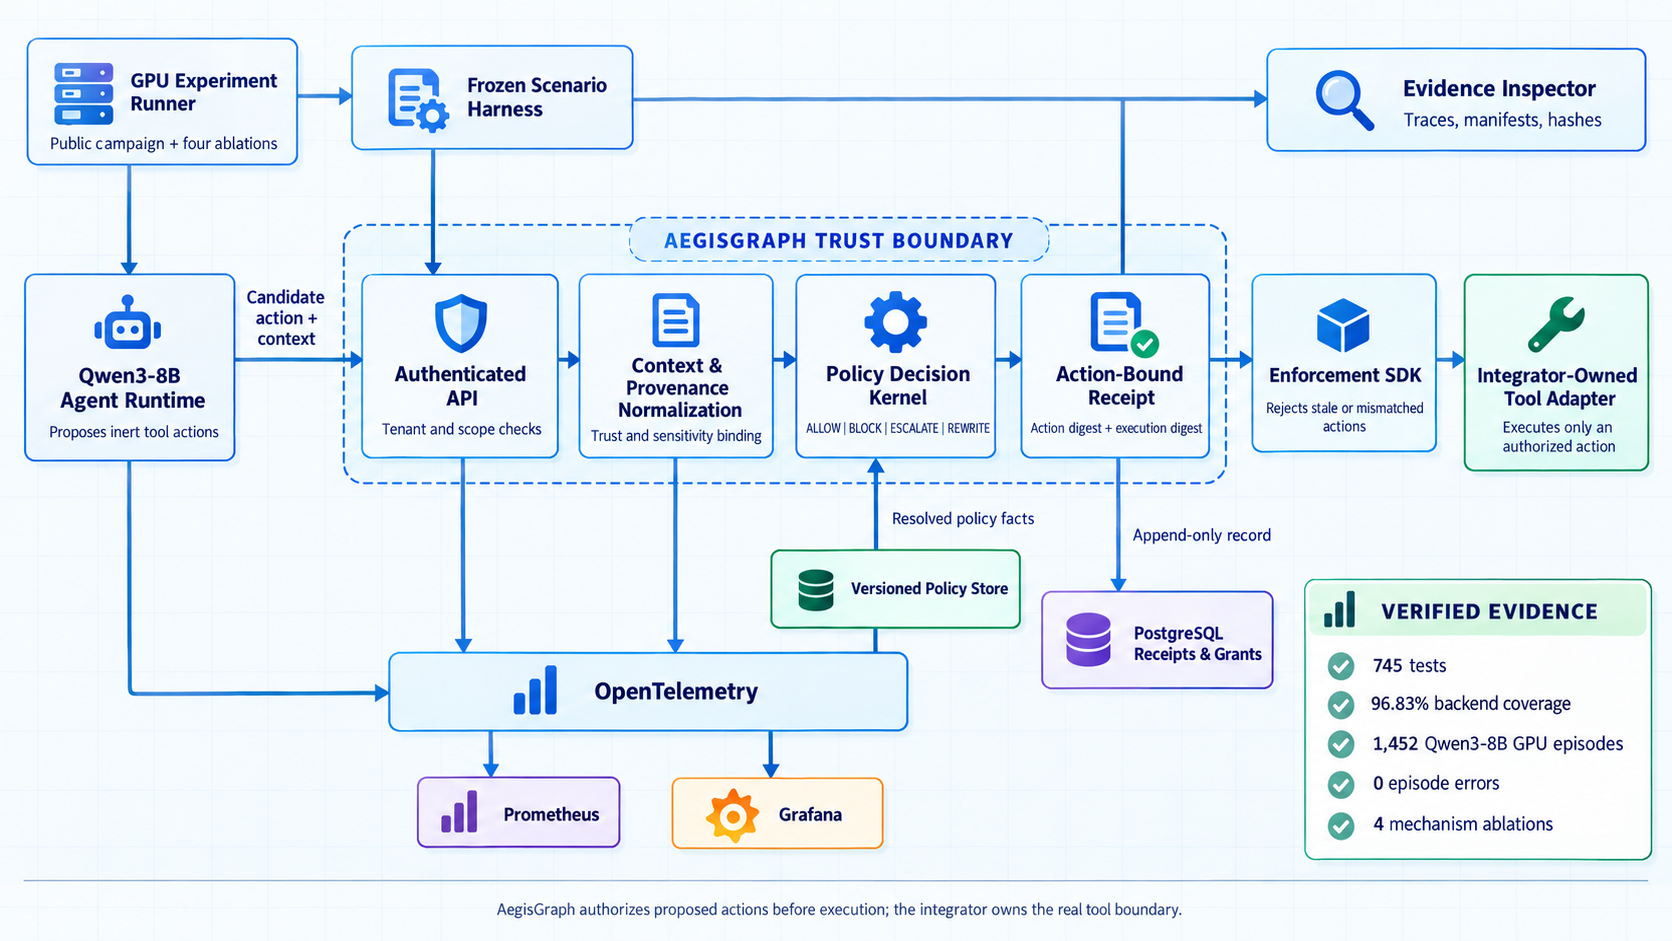
\includegraphics[width=\textwidth]{aegisgraph-architecture.png}
  \caption{Generated architecture of \system. Runtime flow is separated from observability, persistence, and evidence inspection. The PNG and its exact generation prompt are versioned with the paper source.}
  \label{fig:architecture}
\end{figure*}

\subsection{Context and Provenance Normalization}
Inputs arrive through an authenticated API. The normalizer produces a canonical representation of user intent, candidate tool call, contextual evidence, provenance, principal, and deployment metadata. Canonicalization ensures that the same semantic action is hashed consistently and that policy rules do not depend on incidental serialization choices.

\subsection{Policy Decision Kernel}
The decision kernel evaluates explicit, versioned rules and emits a closed decision vocabulary. \textsc{Block} rejects the proposal. \textsc{Escalate} requires an approval or grant. \textsc{Rewrite} produces a constrained argument set that must be used downstream. \textsc{Allow} authorizes the canonical proposal under the receipt's validity conditions. Structured evidence records matched rules, policy revision, and decision reason.

\subsection{Receipts and Enforcement}
The receipt binds the authorization to the canonical principal, tool, and argument digest. Verification occurs at the adapter rather than solely at the API boundary. This closes the gap in which application code could authorize one call and execute another. PostgreSQL persists receipts and grants, while the SDK offers a narrow integration surface for tool owners.

\subsection{Identity and Observability}
The service validates authenticated principals and associates each decision with a stable trace. OpenTelemetry spans cover ingress, normalization, policy evaluation, receipt issuance, persistence, and enforcement. Prometheus/Grafana views support operational inspection, while JSONL traces and review packets support experiment-level analysis.

\section{Implementation}
The reference implementation uses Python and FastAPI for the gateway, PostgreSQL for durable receipts and grants, and an SDK for enforcement integration. Containers define reproducible service dependencies. CI executes unit and integration checks; database-backed tests verify behavior against PostgreSQL rather than relying only on in-memory substitutes. The evaluation runner uses PyTorch and Hugging Face Transformers to execute Qwen3-8B in BF16 or FP16, with pinned source and model revisions captured in manifests.

The codebase separates policy evaluation, persistence, API schemas, cryptographic binding, telemetry, scenario execution, and artifact production. This modularity enables mechanism ablations without rewriting the runner and makes the industrial service usable independently of the research harness.

\section{Experimental Methodology}
\subsection{Research Questions}
\begin{description}[style=nextline]
  \item[RQ1: Runtime reliability.] Can the complete model-to-gateway-to-executor loop run at campaign scale without episode-level runtime failure?
  \item[RQ2: Evidence integrity.] Does the system preserve action--execution correspondence and produce replayable, machine-readable evidence?
  \item[RQ3: Mechanism isolation.] Can provenance, enforcement, and receipt binding be independently removed under an otherwise frozen protocol?
  \item[RQ4: Industrial readiness.] Are service behavior, persistence, coverage, load, and telemetry exercised through automated checks and recorded runs?
\end{description}

\subsection{Scenarios and Splits}
The scenario corpus contains 60 authored cases: 42 development scenarios and 18 validation scenarios. A separate sealed holdout contains 20 cases. Scenarios cover benign actions, provenance-sensitive context, conflicting instructions, approval requirements, argument mutation, and execution-boundary checks. Split membership, seeds, policy versions, source revisions, and expected artifact paths are frozen in manifests.

\subsection{Model and Runtime}
The primary agent is Qwen3-8B \cite{yang2025qwen3}. Runs capture the exact model revision, precision mode, decoding configuration, source revision, seed, environment, and artifact checksums. Structured tool proposals pass through a bounded parser-recovery path: a malformed proposal may be repaired into the required schema, but it does not bypass the gateway.

\subsection{Campaigns and Ablations}
The public campaign contains 612 episodes. Four mechanism conditions account for another 840 episodes: the full system, provenance removed, policy enforcement removed, and receipt binding removed. The same runner and artifact contract are used across conditions so differences can be attributed to the selected mechanism rather than a changed execution path.

\begin{figure*}[t]
  \centering
  \IfFileExists{figures/aegisgraph-evaluation-pipeline.png}{%
    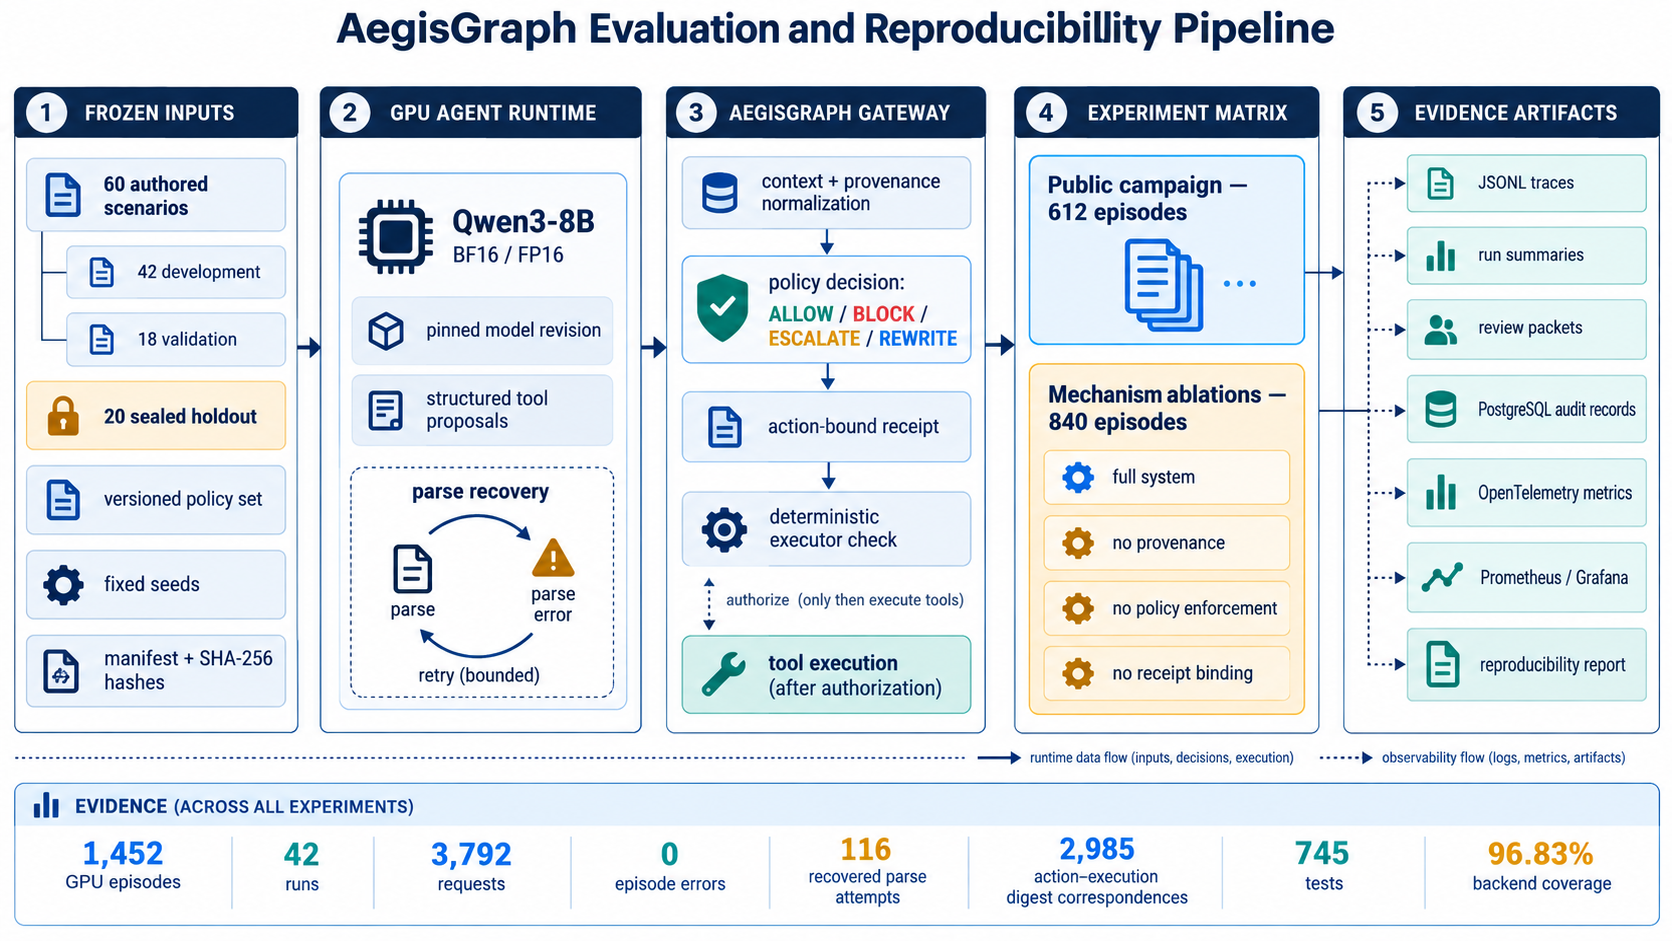
\includegraphics[width=\textwidth]{aegisgraph-evaluation-pipeline.png}%
  }{%
    \fbox{\parbox[c][48mm][c]{0.96\textwidth}{\centering Evaluation pipeline image generated from the prompt in Appendix~\ref{app:prompts}. The final PDF build embeds the PNG artifact.}}%
  }
  \caption{Generated evaluation and reproducibility pipeline. Frozen inputs feed the pinned GPU runtime, gateway, experiment matrix, and evidence package.}
  \label{fig:evaluation}
\end{figure*}

\subsection{Metrics and Artifacts}
Each episode records completion state, parser recovery, gateway requests, decisions, receipt identifiers, action digests, execution digests, trace identifiers, and error state. Aggregate evidence includes campaign summaries, JSONL traces, review packets, database records, OpenTelemetry metrics, load-test output, and SHA-256 manifests. Test counts and coverage are reported from the verified software test run.

\section{Results}
Table~\ref{tab:headline} summarizes the execution-backed evidence. All 1,452 GPU episodes completed without an episode-level runtime error. The 42 runs produced 3,792 gateway requests. The structured-output recovery path repaired 116 parsing attempts, demonstrating that formatting variability could be absorbed without granting execution authority. Across the evaluated paths, 2,985 action--execution digest correspondences were recorded.

\begin{table*}[t]
\centering
\caption{Headline evaluation and engineering evidence. Counts are taken from committed run summaries, manifests, test output, and load artifacts.}
\label{tab:headline}
\small
\begin{tabularx}{\textwidth}{@{}p{0.24\textwidth}p{0.12\textwidth}X@{}}
\toprule
Evidence item & Result & Interpretation \\
\midrule
Qwen3-8B GPU episodes & 1,452 & Complete model-to-gateway episodes across public and ablation campaigns \\
Recorded runs & 42 & Independently materialized run directories and summaries \\
Gateway requests & 3,792 & Requests observed across the evaluated runtime paths \\
Episode-level runtime errors & 0 & Campaigns completed without an episode terminating in runtime error \\
Recovered parse attempts & 116 & Bounded schema recovery preserved the experiment path \\
Action--execution digest correspondences & 2,985 & Authorization and executor evidence shared the recorded digest \\
Automated tests & 745 & Backend, contract, SDK, CLI, integration, and regression coverage \\
PostgreSQL integration tests & 12 & Durable persistence behavior exercised against PostgreSQL \\
Backend statement coverage & 96.83\% & Coverage reported by the verified backend test run \\
Load requests & 2,986 & Measured service requests in the recorded load exercise \\
Load throughput & \mbox{148.938 req./s} & Observed throughput for the recorded configuration \\
\bottomrule
\end{tabularx}
\end{table*}

\begin{table}[t]
\centering
\caption{Experiment allocation.}
\label{tab:allocation}
\small
\begin{tabular}{@{}lr@{}}
\toprule
Campaign & Episodes \\
\midrule
Public evaluation & 612 \\
Mechanism ablations & 840 \\
\midrule
Total & 1,452 \\
\bottomrule
\end{tabular}
\end{table}

\subsection{RQ1: Runtime Reliability}
The zero-error completion result covers the entire 1,452-episode GPU campaign rather than a mocked model path. Parser recovery occurred in 116 attempts, so the absence of episode errors does not imply uniformly perfect model formatting; it shows that the bounded recovery contract handled those cases while preserving authorization checks.

\subsection{RQ2: Evidence Integrity}
The run package links proposals, policy decisions, receipts, executor checks, and traces. The 2,985 recorded action--execution correspondences provide direct evidence that the executor observed the digest associated with authorization. Manifests and checksums make each campaign auditable without depending on a prose-only result summary.

\subsection{RQ3: Mechanism Isolation}
The four-condition ablation matrix executes the same frozen protocol while selectively disabling provenance, policy enforcement, or receipt binding. This turns architectural claims into testable mechanisms and preserves per-episode traces for task-level and security review.

\subsection{RQ4: Industrial Evidence}
The service baseline combines 745 automated tests, 12 PostgreSQL integration tests, and 96.83\% backend coverage. A recorded load run completed 2,986 requests at 148.938 requests/s with zero reported request errors. Traces and metrics connect service behavior to Prometheus/Grafana-compatible operational views.

\section{Discussion}
\paragraph{Authorization outside the model.} The central design choice is to prevent fluent model output from serving as authority. The model can propose and explain; the gateway decides under explicit policy; the adapter verifies the resulting capability immediately before the side effect.

\paragraph{Evidence as a product surface.} Receipts, traces, manifests, and review packets are not secondary logs. They form the interface by which a security reviewer can reconstruct why an action was permitted, whether it changed before execution, and which policy version governed the decision.

\paragraph{Research--engineering alignment.} The same service path is used by the GPU experiments and the industrial stack. This avoids a common gap in which a research-only detector is evaluated separately from the code that would enforce it. Ablations are configuration-controlled variations of the deployed mechanism boundary.

\section{Reproducibility Statement}
The repository includes scenario definitions, split manifests, pinned runtime configuration, fixed seeds, container definitions, policy versions, evaluation scripts, machine-readable traces, run summaries, review packets, and evidence documentation. Public claims are attached to concrete artifact paths. GPU runs record both the project revision and the model revision. The paper source, generated figures, and exact figure prompts are versioned beside the implementation.

To reproduce the study, an evaluator prepares the declared Python environment, provisions PostgreSQL, starts the gateway, runs the verified test suite, and launches the frozen Qwen3-8B campaign under the provided manifest. The evidence builder then validates expected files and hashes before producing aggregate summaries. Hardware-dependent throughput should be interpreted together with the recorded environment and configuration.

\section{Scope and Validity}
The reported results establish the behavior of the committed scenarios, policies, model configuration, service stack, and experiment artifacts. The evaluation separates execution-backed quantities from semantic judgments: runtime completion, request counts, receipt correspondence, tests, coverage, and load evidence are mechanically derived; task utility and adversarial success require the declared review procedure. This separation keeps the public claims traceable and provides a stable basis for later blinded annotation, additional models, adaptive attacks, and cross-domain scenarios.

\section{Ethics and Responsible Use}
\system is defensive infrastructure for constraining and auditing tool-using agents. The released scenarios and traces are intended to improve authorization design, evaluation quality, and incident analysis. Deployers should minimize sensitive data in traces, apply retention controls to receipts and grants, protect signing material, and require explicit human approval for high-impact actions where policy calls for escalation.

\section{Conclusion}
\system introduces an action-bound policy and evidence gateway for tool-using LLMs. Its explicit decision vocabulary, provenance-aware normalization, versioned policies, executor-side receipt verification, and traceable evidence package move authority away from untrusted model text and into an auditable system boundary. The implementation is supported by 1,452 Qwen3-8B GPU episodes, four mechanism conditions, 3,792 gateway requests, zero episode-level runtime errors, 745 automated tests, 96.83\% backend coverage, and recorded load evidence. The project provides both a research instrument for studying agent security mechanisms and an industrial foundation for integrating enforceable controls into real tool adapters.

\footnotesize
\begin{thebibliography}{9}
\bibitem{yao2023react}
S. Yao, J. Zhao, D. Yu, N. Du, I. Shafran, K. Narasimhan, and Y. Cao.
\newblock ReAct: Synergizing Reasoning and Acting in Language Models.
\newblock \emph{ICLR}, 2023. arXiv:2210.03629.

\bibitem{greshake2023indirect}
K. Greshake, S. Abdelnabi, S. Mishra, C. Endres, T. Holz, and M. Fritz.
\newblock Not What You've Signed Up For: Compromising Real-World LLM-Integrated Applications with Indirect Prompt Injection.
\newblock arXiv:2302.12173, 2023.

\bibitem{ruan2023toolemu}
Y. Ruan, H. Dong, A. Wang, S. Pitis, Y. Zhou, J. Ba, Y. Dubois, C. J. Maddison, and T. Hashimoto.
\newblock Identifying the Risks of LM Agents with an LM-Emulated Sandbox.
\newblock arXiv:2309.15817, 2023.

\bibitem{debenedetti2024agentdojo}
E. Debenedetti, J. Zhang, M. Balunovi\'c, L. Beurer-Kellner, M. Fischer, and F. Tram\`er.
\newblock AgentDojo: A Dynamic Environment to Evaluate Prompt Injection Attacks and Defenses for LLM Agents.
\newblock \emph{NeurIPS}, 2024. arXiv:2406.13352.

\bibitem{debenedetti2025camel}
E. Debenedetti, I. Shumailov, T. Fan, J. Hayes, N. Carlini, D. Fabian, C. Kern, C. Shi, A. Terzis, and F. Tram\`er.
\newblock Defeating Prompt Injections by Design.
\newblock arXiv:2503.18813, 2025.

\bibitem{wallace2024hierarchy}
E. Wallace, K. Xiao, R. Leike, L. Weng, J. Heidecke, and A. Beutel.
\newblock The Instruction Hierarchy: Training LLMs to Prioritize Privileged Instructions.
\newblock arXiv:2404.13208, 2024.

\bibitem{yang2025qwen3}
A. Yang, A. Li, B. Yang, et al.
\newblock Qwen3 Technical Report.
\newblock arXiv:2505.09388, 2025.
\end{thebibliography}

\end{document}
